 \documentclass{beamer}

\usepackage{ucs}
\usepackage[utf8x]{inputenc}
\usepackage[T1]{fontenc}
\usepackage[english]{babel}
\usepackage[retainorgcmds]{IEEEtrantools}%	IEEEeqnarray
\usepackage{mathabx}%	convolution symbol
\usepackage{multi row}
\usepackage{listings}

\usepackage{epstopdf}

\lstset{
	language=C++,
	basicstyle=\footnotesize,
	showtabs=true,
	tabsize=3,
}

%	presentation info
\title{Optimization of a Finite-Volume Method Application}

\author{José Alves, Rui Brito}

\institute[22765, 22781]{
	Universidade do Minho
}

\date{Braga, June 2013}


%	beamer options
\usetheme{CambridgeUS}


\begin{document}%	begin presentation

\maketitle%	title slide

\begin{frame}
	\frametitle{Index}
	\tableofcontents
\end{frame}

\section{Introduction}
\begin{frame}
	\frametitle{conv-diff (Recap)}
	\begin{description}
		\item [What?] Computes the heat diffusion of a fluid spreading over an area;
		\item [How?] Uses a Finite-Volume method;
		\item [Why?] Represents surface as a mesh, making each cell only dependent of its neighbours;
	\end{description}
\end{frame}

\begin{frame}
	\begin{figure}[!htp]
    	\centering   
        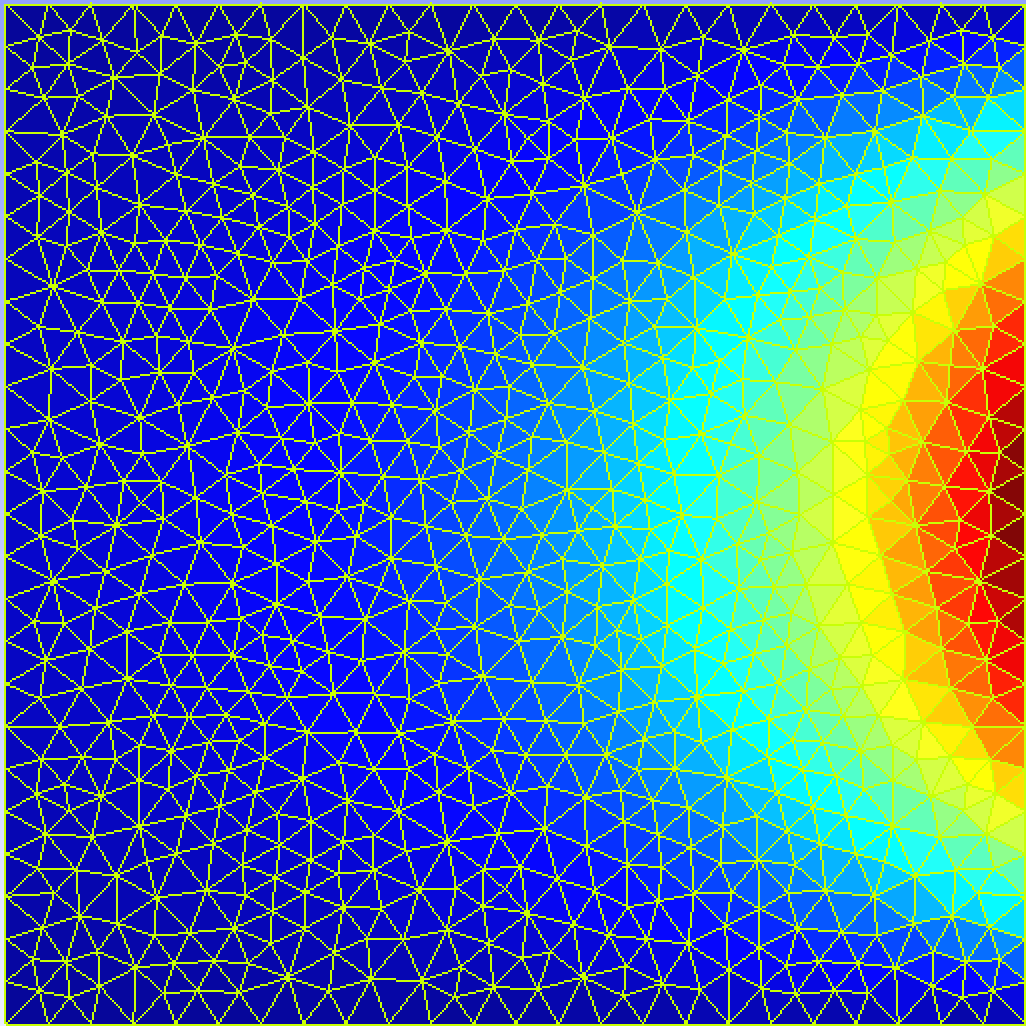
\includegraphics[width=.6\textwidth]{../images/mesh.png}        
	\end{figure}
\end{frame}

\begin{frame}
	The main objective is to compute a vector $\overline{\phi}$ such that $\overline{\phi} \longrightarrow G(\overline{\phi}) = \left(\begin{array}{c}
	0\\ 
	0\\
	\vdots\end{array}\right)$
	This is accomplished in three different stages:
	\begin{enumerate}
	    \item {We begin with a candidate vector $\phi$} 
	    \item {For each edge, we compute the flux $F_{ij}$, with $i$ and $j$ being the indexes of the adjacent cells}
	    \item {For each cell, we compute $\sum |e_{ij}| F_{ij} - |c_i| f_i$}
	\end{enumerate}
	Thus: $\phi = \left(\begin{array}{c}
	\phi_1\\
	\vdots\\
	\phi_I
	\end{array}\right) \longrightarrow G = \left(\begin{array}{c}
	G_1\\
	\vdots\\
	G_I
	\end{array}\right)$
\end{frame}

\begin{frame}
	\begin{description}
		\item [makeFlux] Compute the contribution from each edge;
		\item [makeResidual] Compute the $\phi$ vector, adding the flux for each cell from each contribution;	
	\end{description}
\end{frame}

\section{Original Implementation}

\begin{frame}
	\frametitle{Original implementation}
	\begin{itemize}
		\item \textbf{\itshape Arrays-of-Pointers};				
	\end{itemize}

	\begin{columns}
		\column{.45\textwidth}		
		\begin{block}{makeFlux}
			
			For all \textbf{edges}:
			\begin{enumerate}
				\item Read adjacent cell data;	
				\item Compute edge velocity;
				\item Compute flux through edge;				
			\end{enumerate}
		\end{block}

		\column{.45\textwidth}		
		\begin{block}{makeResidual}
			
			For all \textbf{edges}:
			\begin{enumerate}
				\item Subtract flux from right cell;
				\item Add flux to left cell;
			\end{enumerate}
		\end{block}
	\end{columns}
\end{frame}

\section{Optimizations}

\begin{frame}
	\frametitle{Naive Optimizations}	
		\begin{itemize}
		\item Removed redundant loads and calculations;
		\item Changed some variable definitions to \emph{const};
		\item Usage of a recent compiler auto-optimizations(SLP);				
	\end{itemize} 	
\end{frame}

\begin{frame}
	\frametitle{OpenMP}
\end{frame}

\begin{frame}
\titlepage
	\begin{center}
		\Huge\bfseries
		- ? -
	\end{center}
\end{frame}

\end{document}%	end presentation